%%
%% In this section:
%%
%%   - explain stream setting, problems and objectives/aims
%%   - theoretical frameworks?
%%   - stream processes, continuous systems
%%   - Frameworks
%%        - batch processing: RM, Weka
%%        - mini-batches + parallelization:  MapReduce,Hadoop,Radoop
%%        - stream processing: moa,s4.io,storm,Streams-Plugin
%%
%%   - ggf. �bersichtstabelle mit den Ans�tzen und Einordnen des Streams Plugin?
%%
%% (  - refine the basic problems and task/settings we want to address )
%% (  - give an overview of existing frameworks/solutions )
%% (  - outline the differences of the streams library to this solutions )
%%
\section{\label{sec:relatedWork}Problem and Related Work}
The traditional batch data processing aims at computations on fixed
chunks of data in one or more passes. The results of these
computations again form a fixed outcome that can further be used as
input. A simple example is given by the computation of a prediction
model based on some fixed training set. After the determination of a
final model, the learning step is finished and the model is applied to
deliver predictions based on the learning phase. Similar situations
arise for the computation of statistics, creation of histograms, plots
and the like. From a machine learning perspective, this has been the
predominant approach of the last years.

Two aspects have been changed in the data we are facing today, which
requires a paradigm shift: The size of data sets has grown to amounts
intractable by existing batch approaches, and the rate at which data
changes demands for short-term reactions to data drifts and updates of
the models.

\subsection{Processing Masses of Data}
The former problem has been addressed by massive parallelism. With the
drop of hardware prizes and evolving use of large cloud setups,
computing farms are deployed to handle data at a large scale. Though
parallelism and concepts for cluster computing have been studied for
long, their applicability was mostly limited to specific use
cases. 

One of the most influential works to use computing clusters in data
analysis is probably Google's revival of the {\em map-and-reduce}
paradigm \cite{googleMapReduce}. The concept has been around in
functional programming for years and has now been transported to
large-scale cluster systems consisting of thousands of compute
nodes. Apache's open-source {\em Hadoop} implementation of a
map-and-reduce platform nowadays builds a foundation for various
large-scale systems.

With the revival of map-and-reduce, various machine learning algorithms
have been proven to be adjustable to this new (old) way of computing.

%In the massive parallel settings, we are given a large set of examples
%$\mathbf{X} \subseteq \mathbb{R}^p$. Models on this data are typically
%computed by partitioning the data, computing intermediate results
%({\em map} phase) and merging these results to a final output ({\em
%  reduce} phase) as shown in Figure \ref{fig:mapReduce}.
%
%\begin{figure}[ht!]
%  \begin{center}
%        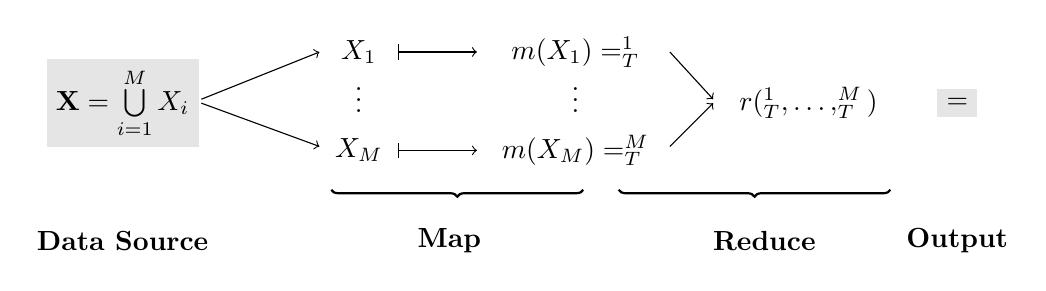
\begin{tikzpicture}
      \draw (-2.5,0.35) node[rectangle,fill=black!10] { $\mathbf{X} = \bigcup\limits_{i=1}^M X_i$ };
      \draw (-2.5,-1.4) node {\textbf{Data Source}};

      \draw[->] (-1.5,0.4) -- (0,1);
      \draw[->] (-1.5,0.35) -- (0,-0.2);

      \draw (0.5,1) node[rectangle] {$X_1$};
      \draw (0.5,-0.25) node[rectangle] {$X_M$};

      \draw (0.5,0.5) node {$\vdots$};


      \draw[|->] (1,1) -- (2,1);
      %\draw (1.5,1.25) node {$m$};
      \draw (3.25,1) node {$m(X_1) = \barw_T^1$}; %X_1'

      \draw[|->] (1,-0.25) -- (2,-0.25);
      %\draw (1.5,0) node {$m$};
      \draw (3.25,-0.25) node {$m(X_M) = \barw_T^M$}; %X_M'

      \draw (3.25,0.5) node {$\vdots$};

      %\draw (2,-0.25) node[rectangle,draw=black] {$m(X_M)$};

      \draw[->] (4.45,1) -- (5,0.4);
      \draw[->] (4.45,-0.2) -- (5,0.35);

      %\draw (6.21,0.35) node {$r(X_1',\ldots,X_M')$};
      \draw (6.21,0.35) node {$r(\barw_T^1,\ldots,\barw_T^M)$};

      \draw[decorate,decoration={brace, mirror},thick] (0.15,-0.75) -- (3.35,-0.75); % node at (6.5,-.5) {}; 
      \draw (1.65,-1.4) node {\textbf{Map}};

      \draw[decorate,decoration={brace, mirror},thick] (3.8,-0.75) -- (7.25,-0.75); % node at (6.5,-.5) {}; 
      \draw (5.65,-1.4) node {\textbf{Reduce}};

      \draw (8.1,0.35) node[rectangle,fill=black!10] {$=\barbarw$}; %$\ \overline{w}$.
      \draw (8.1,-1.4) node {\textbf{Output}};

    \end{tikzpicture}

%    \caption{\label{fig:mapReduce}The map-and-reduce paradigm.}
%  \end{center}
%\end{figure}


%%
%% Beispiele fuer Lerner die Map&Reduce f�hig sind
%%  - Ensemble,...
%%  -
%% Software: Mahout,... andere?
%%

\subsection{The Problem of Continuous Data}
Whereas the massive parallelism addresses the batch computation of
large volumes of data, it still requires substantial processing time
to re-compute prediction models, statistics or indexes once data has
been changed. Therefore it does not fully reflect the demands for
reacting to short-term drifts of data.

Within this work we will refer to this as the setting of {\em
  continuous data}, i.e. we consider an unbound source $D$ of data
that continuously emits data items $d_i$. In the following, we model
that data stream as a sequence
$$D = \langle d_0,d_1,\ldots,d_i,\ldots \rangle$$
with $i\rightarrow\infty$. At any time $t$ we want to provide some
model that reflects the analysis of the items $d_i$ with $i\le t$.
Typical tasks to compute on $S$ are
\begin{itemize}
\item Given $d_i \in \mathbb{N}$ - finding the top-$k$ most frequent
  values observed until $t$.
\item For $d_i \in \mathbb{N}^p$ - find the item sets $I \subset
  \mathbb{N}^p$ which most frequently occurred in the $d_i$.
\item With $d_i \subset X$, provide a classifier $c:X \rightarrow Y$,
  that best approximates the real distribution of labeled data $X
  \times Y$ (classification).
\item Provide a clustering $C$ for the data item $d_i$ observed so far (clustering).
\item Find indications on when the overall distribution of the $d_i$
  changes within the stream (concept drift detection).
\end{itemize}
Often, these tasks are further refined to models that focus on a
recent sliding window of the last $w$ data items observed, e.g. we are
interested in the top-$k$ elments of the last 5 minutes. 

Algorithms for solving these tasks on static data sets
exists. However, the challenging requirements in the continuous data
setting are the tight limits on the resources available for
computation. This can for example be realtime constraints, such as a
fixed limit on the time available for processing a data item, or a
bound on the memory available for computation.

%
%. The {\em data items} $s_i$ are tuples of
%$M^p$ with $p \ge 1$ where $M^p = M_1 \times \ldots \times M_p$ for
%any sets $M_j$. 
%
%The $M_j$ can be any discrete sets of a fixed domain as well as $M_k
%\subseteq \mathbb{R}$. The index $i$ may reflect some time unit or an
%(monotonically increasing) time like dimension, constituting the
%sequence of tuples. For $p=1$ and $M_1 = \mathbb{R}$ this models a
%single value series with index $i$.
%The data processing model of streaming approaches share common
%criteria.
% induced by the continuous nature of the problem. 
The framing to operate on streaming data is generally given by the
following constraints/requirements:
\begin{itemize}
  \defitem{C1} continuously processing {\em single items} or {\em small batches} of data,
  \defitem{C2} using only a {\em single pass} over the data,
  \defitem{C3} using {\em limited resources} (memory, time),
  \defitem{C4} provide {\em anytime services} (models, statistics).
\end{itemize}

Several algorithms to the task mentioned above with respect to these
requirements have been proposed. Regarding the counting of elements
and sets of items, a variety of different approximate count algorithms
based on sketches of the data have been developed in
\cite{Charikar02findingfrequent,goethals2007,Cheng06maintainingfrequent}.
For statistical model, estimators for quantiles have been presented in
\cite{Greenwald/Khanna/2001a,Arasu/Manku/2004a}.



\bigskip

Whereas a wide range of different methods have been provided for
various streaming tasks, this work aims at providing an abstract
framework to integrate these different approaches into a flexible
environment to build a streaming analysis based upon the existing
algorithms.

%%The examples outlined above show typical use cases of high-volume
%%continues data that is either stored in large batches (e.g. 5-minute
%%recording intervals of the FACT telescope) or continuously produced
%%by non-terminating processes.
%%
%%The results is a sequence of 150 images (slices), each containing 1440
%%pixels.  As the shower is not clearly identifiable, a {\em region of
%%  interest} of about 300 slices is recorded, which results in 432000
%%raw data values for a single shower (event). 
%%
%%Currently showers are recorded at a rate of 60 Hz, resulting in 60 of
%%such events being stored each second. With additional information for
%%each shower, a 5 minute recording interval quickly produces several
%%gigabytes of raw data that is to be preprocessed and analyzed.
%%
%With nowadays data volume, the traditional batch processing model
%quickly reaches the resource limitations of single workstations. Even
%applying a previously created prediction model to a large set of
%examples can quickly become impossible if the example set itself does
%not fit into main memory. The only cumbersome solution often is to
%split the data into several files and process each file separately.
%We will refer to this setting as the {\em partial batch processing}.
%This processing typically requires the results of the processed
%batches to be combined, for example by computing an average.
%
%In some cases, the data is not even static, but continuosly produced
%by some data generating process. In the simplest case we might be able
%to write batches of that data into files and fall back to the mini
%batch processing approach. Therefore in this work we are more
%interested in continuously processing that data and provide models or
%services in an {\em anytime} manner, that is the current models or
%statistics can be queried at any time. We will refer to this setting
%as the ({\em continuous}) {\em stream processing}.  When dealing with
%a finite source of data we can consider the {\em stream processing} as
%a special case of {\em partial batch processing} with a batch size of 1.
%
%The data processing model of streaming approaches share common
%criteria.
% induced by the continuous nature of the problem. 
%The framing to operate on streaming data is generally given by the
%following constraints/requirements:
%\begin{itemize}
%  \item[\textsf{C1}] continuously processing {\em single items} or {\em small batches} of data,
%  \item[\textsf{C2}] using only a {\em single pass} over the data,
%  \item[\textsf{C3}] using {\em limited resources} (memory, time),
%  \item[\textsf{C4}] provide {\em anytime services} (models, statistics).
%\end{itemize}
%This contrasts to the RapidMiner batch-processing model, where a set
%of examples is usually processed in its entirety and during a single
%execution of a RapidMiner process.


\subsection*{Existing Frameworks}
%Various frameworks exist that support either of these two processing
%modes.
Parallel batch processing is addressing the setting of fixed data and
is of limited use if data is non-stationary but continuously produced,
for example in monitoring applications (server log files, sensor
networks).  A framework that provides online analysis is the MOA
library \cite{moa}, which is a Java library closely related to the
WEKA data mining framework \cite{weka}. MOA provides a collection of
online learning algorithms with a focus on evaluation and
benchmarking.

Aiming at processing high-volume data streams two environments have
been proposed by Yahoo! and Twitter. Yahoo!'s {\em S4} \cite{s4io}
as well as Twitter's {\em Storm} \cite{storm} framework do provide
online processing and storage on large cluster infrastructures, but
these do not include any online learning.

In contrast to these frameworks, the \streams library focuses on
defining a simple abstraction layer that allows for the definition of
stream processes which can be mapped to different backend
infrastructures (such as {\em S4} or {\em Storm}).

%Providing an execution environment for data stream processing is given
%in s4.io \cite{s4io} and {\em storm} \cite{storm}. These libraries
%... \todo{More details about s4io/storm}.

